
% np.sqrt()
% np.round( , num_decimals)
% np query syntax
% np.append
% np.flip
% two kinds of sorting
% remove (by index  and by value?)

% indexing, slices

\chapter{Arrays in Python (2 of 2)}
\label{ch:arraysInPython2}

\index{array!in NumPy}
\index{ndarray@\texttt{ndarray} (NumPy)}

Now that we know several options for how to \textit{create} \texttt{ndarrays},
what can we do with them? Many and sundry things.

\section{Getting the array size}

To learn how long an array is (\textit{i.e.}, how many elements) we use the
\texttt{len()} function, kind of like we did for strings. Refer back to
Figure~\ref{fig:arraysInMemory} (p.~\pageref{fig:arraysInMemory}) and consider
this code:

\begin{Verbatim}[fontsize=\footnotesize,samepage=true,frame=single,framesep=3mm]
num_players = len(roster)
big_number = len(photo_likes)
print("There are {} players on the USWNT.".format(num_players))
print(big_number)
print("We've had {} elections.".format(len(prez_elections)))
\end{Verbatim}

\begin{Verbatim}[fontsize=\footnotesize,samepage=true,frame=single,framesep=3mm]
There are 24 players on the USWNT.
40000000000
We've had 59 elections.
\end{Verbatim}

\index{overloading}
\index{return@``returning'' a value}
\index{array!length}
\index{len@\texttt{len()}}
\index{element}
This is an example of Python \textbf{overloading} function names, which just
means that the same name is used for two different functions. When you pass a
string to \texttt{len()}, you get the number of characters; but when you pass
an array to \texttt{len()}, you get the number of elements it has.
(The \texttt{roster} array had way more than 24 \textit{letters} in it, notice
-- but \texttt{len()} returned 24 since that was the number of strings.)

\section{Accessing individual elements}

\subsection{Retrieving an element}

\index{boxies (square brackets)}
\index{[]@\texttt{[]} (boxies)}
\index{element}
To get the value of a specific element from an array, we use ``boxie notation''
with the index number:

\begin{Verbatim}[fontsize=\small,samepage=true,frame=single,framesep=3mm]
print(prez_elections[0])
third_year = usa_years[2]
print("{} was the 3rd year of U.S.A.".format(third_year))
print("The highest-numbered player is {}".format(
    roster[len(roster)-1]))
\end{Verbatim}

\begin{Verbatim}[fontsize=\small,samepage=true,frame=leftline,framesep=5mm,framerule=1mm]
1788.0
1778 was the 3rd year of U.S.A.
The highest-numbered player is Christen Press.
\end{Verbatim}

Remember, indices start at zero (not one) so that's why the first line has a
\texttt{0} in it.

Now examine that last line, which is kind of tricky. Whenever you have boxies,
you have to first evaluate the code \textit{inside} them to get a number. That
number is then the index number Python will look up in the array. In the last
line above, the code \textit{inside} the boxies is:

\quad\quad\quad   ...\texttt{len(roster)-1}...

Breaking it down, we know that \texttt{len(roster)} is 24, which means
\texttt{len(roster)-1} must be 23, and so \texttt{roster[len(roster)-1]} is
\texttt{Christen Press}. It's a common pattern to get the last element of an
array.\footnote{Fun fact: you can also use \textit{negative} indices to mean
``from the end of the array, rather than the beginning.'' So
\texttt{roster[-1]} will also give you \texttt{Christen Press},
\texttt{roster[-2]} is \texttt{Jessica McDonald},
\texttt{roster[-5]} is \texttt{Crystal Dunn}, \textit{etc.} (see
p.~\pageref{rosterNames} for the values). I find this a bit obscure, though, so
I don't normally use this feature. (Negative indices also mean a completely
different thing in the R language, which is another reason I eschew them in
both R and Python.)}

To test your understanding, figure out what the following code will print:

\label{indexTest}
\begin{Verbatim}[fontsize=\small,samepage=true,frame=single,framesep=3mm]
q = 2
r = np.array([45,17,39,99])
s = 1
print(r[q-s+1]+3)
\end{Verbatim}

The answer is at the end of the chapter.

\subsection{Changing an element}

To modify an element of an array, just use the equals sign like we do for
variables:

\index{stooges@Stooges (The Three)}
\index{beavis@Beavis}
\begin{Verbatim}[fontsize=\small,samepage=true,frame=single,framesep=3mm]
stooges = np.array(['Larry','Beavis','Moe'])
print(stooges)
stooges[1] = 'Curly'
print(stooges)
\end{Verbatim}

\begin{Verbatim}[fontsize=\small,samepage=true,frame=leftline,framesep=5mm,framerule=1mm]
['Larry' 'Beavis' 'Moe']
['Larry' 'Curly' 'Moe']
\end{Verbatim}

After all, an individual element like \texttt{stooges[1]} is itself a variable
pretty much like any other.

% Omit: slices

\section{``Vectorized'' arithmetic operators}

Recall our table of Python math operators (Figure~\ref{fig:mathOps} on
p.~\pageref{fig:mathOps}). What do those things do if we use them on aggregate,
instead of atomic data? The answer is: something super cool and useful.

\subsection{Operating on an array and a single value}

Consider the following code:

\label{vectorizedArrayIntExample}
\begin{Verbatim}[fontsize=\small,samepage=true,frame=single,framesep=3mm]
num_likes_today = np.array([6,61,0,0,14])
num_likes_tomorrow = num_likes_today + 3
print(num_likes_tomorrow)
\end{Verbatim}

\begin{Verbatim}[fontsize=\small,samepage=true,frame=leftline,framesep=5mm,framerule=1mm]
[ 9 64 3 3 17 ]
\end{Verbatim}

See what happened? ``Adding 3'' to the \textit{array} means adding 3 \textit{to
each element}. All in one compact line of code, we can do five -- or even five
billion -- operations. This works for all the other Figure~\ref{fig:mathOps}
operators as well.

\index{vectorized@``vectorized'' operation}

For somewhat geeky reasons, this sort of thing is called a \textbf{vectorized}
operation. All you need to know is that this means \textbf{fast}. And that's
``fast'' in two different ways: fast to write the code (since instead of using
a \textbf{loop}, which we'll cover in \ref{ch:loops}, you just write a single
statement with \texttt{+} and \texttt{=} signs), and more importantly, fast to
\textit{execute}. For more geeky reasons, the above code will run lightning
fast even if \texttt{num\_likes\_today} had five hundred million elements
instead of just five. As you'll learn if you ever try it, a Python loop is much
slower.\footnote{I just ran that comparison on my laptop, and here are the
results. Using the plain-ol' ``\texttt{+}'' vectorized operator, my machine
added the number 3 to an array with five hundred million elements in just 1.51
seconds. A loop, by contrast, took 2.8 \textit{minutes} to do the same thing.}

Don't get me wrong: there are times we'll have to use a loop because we have no
choice. But the general rule with Python is: if you can figure out how to
perform a calculation without using a loop, always do it!


\subsection{Operating on two arrays}

\index{vectorized@``vectorized'' operation}

Possibly even cooler, we can even ``\texttt{+}'' (or ``\texttt{-}'', or
``\texttt{*}'', or...) two entire \textit{arrays} together. Example:

\label{vectorizedArrayArrayExample}
\begin{Verbatim}[fontsize=\small,samepage=true,frame=single,framesep=3mm]
salaries = np.array([38000, 102000, 55750, 29500, 250000])
raises = np.array([1000, 4000, 2000, 1000, 2000])
salaries = salaries + raises
print(salaries)
\end{Verbatim}

This code produces:

\begin{Verbatim}[fontsize=\small,samepage=true,frame=leftline,framesep=5mm,framerule=1mm]
[ 39000 106000 57750 30500 252000]
\end{Verbatim}

Can you see why? ``Adding'' the two arrays together performed addition
\textit{element-by-element}. The result is a new array with $38000+1000$ as the
first element, $102000+4000$ as the second, \textit{etc.} This, too, is a
lightning-fast, vectorized operation, and it too works with all the other math
operators.

Just to re-emphasize one point before we go on. In the example back on
p.~\pageref{vectorizedArrayIntExample}, we assigned the result of the operation
to a new variable, \texttt{num\_likes\_tomorrow}. This means that
\texttt{num\_likes\_today} itself was \textit{unchanged} by the code. In
contrast, in the example we just did, we assigned the result of the operation
back into an \textit{existing} variable (\texttt{salaries}). So
\texttt{salaries} has itself been updated as a result of that code.

% TODO: could include memory picture to this effect.


\section{Copying -- and \textit{not} copying -- arrays}

\label{copyingNotCopyingArrays}
\index{copying@copying (arrays)}
Now, a surprise for the unwary. Suppose I write this code:

\label{code:refNotCopy}
\begin{Verbatim}[fontsize=\small,samepage=true,frame=single,framesep=3mm]
stooges = np.array(['Larry','Beavis','Moe'])
funny_people = stooges
stooges[1] = 'Curly'
print("The stooges are: {}.".format(stooges))
print("The funny people are: {}.".format(funny_people))
\end{Verbatim}

Take a moment and predict what you think the output will be. Then, read it and
(possibly) weep:

\begin{Verbatim}[fontsize=\small,samepage=true,frame=leftline,framesep=5mm,framerule=1mm]
The stooges are: ['Larry' 'Curly' 'Moe'].
The funny people are: ['Larry' 'Curly' 'Moe'].
\end{Verbatim}

Note carefully: \textit{no \texttt{Beavis}}.

\begin{figure}[ht]
\centering
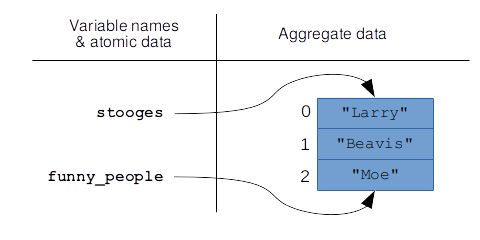
\includegraphics[width=0.49\textwidth]{refNotCopy.png}
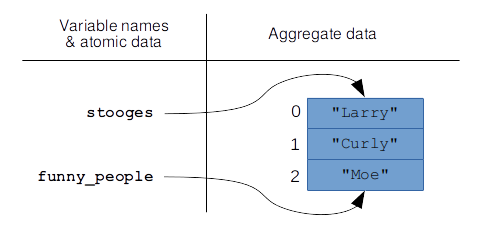
\includegraphics[width=0.49\textwidth]{refNotCopy2.png}
\caption{The code on p.~\pageref{code:refNotCopy} immediately before (left
side) and after (right side) the line ``\texttt{stooges[1] = \textquotesingle
Curly\textquotesingle}'' is reached.}
\label{fig:refNotCopy}
\end{figure}

\index{memory!picture}

Now the question is why. To understand this (and virtually any other tricky
programming problem) you have to return once again to the memory picture.
Figure~\ref{fig:refNotCopy} shows the situation immediately before, and after,
the line ``\texttt{stooges[1] = \textquotesingle Curly\textquotesingle}''
executes. Crucially, \textit{there is only one array} in memory. Both variables
-- \texttt{stooges} and \texttt{funny\_people} -- are pointing at it.

You see, if \texttt{y} contains \textit{aggregate} (instead of atomic) data,
the line ``\texttt{x = y}'' does not perform a copy operation. Instead, it just
points the \texttt{x} variable name to the same place \texttt{y} is pointing
to.

Once you grasp this, it's easy to see why \texttt{"Beavis"} completely
disappeared. There's only one array at all, so changing \texttt{stooges} has
the side effect of implicitly changing \texttt{funny\_people} as well.

\subsection{Actually copying}

The ``point the variable to the same thing, but don't do a copy'' behavior is
the default, because such copy operations are expensive (in terms of memory
usage and time to execute). They're normally not what you want anyway.
Sometimes, however, you \textit{do} want to produce an entire separate copy of
an array, so you can modify the copy yet preserve the original. To do so, you
use the \texttt{.copy()} method:

\begin{Verbatim}[fontsize=\footnotesize,samepage=true,frame=single,framesep=3mm]
orig_beatles = np.array(['John', 'Paul', 'George', 'Pete'])
beatles = orig_beatles.copy()
beatles[3] = 'Ringo'
print("The Beatles were originally {}.".format(orig_beatles))
print("But the ones we all know were {}.".format(beatles))
\end{Verbatim}

Look carefully at that second line: it makes all the difference. Instead of
making the new variable \texttt{beatles} point to the same array in memory that
\texttt{orig\_beatles} did, we explicitly copied the array and made
\texttt{beatles} point to that new copy. The final memory picture is thus as
per Figure~\ref{fig:copyNotRef}, and the output is of course:

\begin{Verbatim}[fontsize=\footnotesize,samepage=true,frame=leftline,framesep=5mm,framerule=1mm]
The Beatles were originally ['John' 'Paul' 'George' 'Pete'].
But the ones we all know were ['John' 'Paul' 'George' 'Ringo'].
\end{Verbatim}

\begin{figure}[ht]
\centering
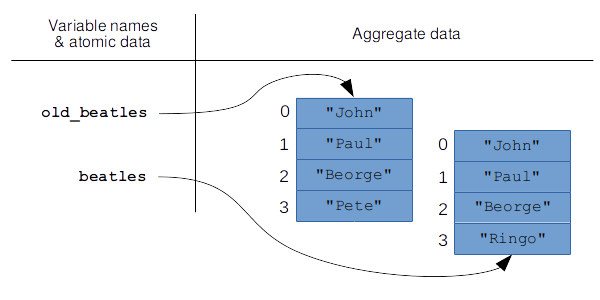
\includegraphics[width=0.9\textwidth]{copyNotRef.png}
\caption{The memory picture after calling the \texttt{.copy()} method, instead
of simply assigning to a new variable.}
\label{fig:copyNotRef}
\end{figure}


\section{Sorting arrays}

\label{sortingArrays}
\index{sorting@sorting (arrays)}
\index{int@\texttt{int}}
\index{float@\texttt{float}}
\index{str@\texttt{str}}
A common operation in Data Science is to \textbf{sort} an array, either
numerically (if the array contains \texttt{int}s or \texttt{float}s) or
alphabetically (if it contains strings). There are two ways to do this, which
turn out to differ in exactly the same was as the operations in the previous
section.

\index{on@``on''}
\index{sort@\texttt{.sort()}}
\index{in place@``in place''}
\index{calling a method@``calling'' a method (on a variable)}
One way is to call the \texttt{.sort()} method directly \textbf{on} an array.
This sorts the array \textbf{in place}, which means that the actual data in
memory is rearranged right then and there. As an important side effect, any
\textit{other} variable that points to the same array will \textit{also} be
sorted.

Here's an example:

\begin{Verbatim}[fontsize=\small,samepage=true,frame=single,framesep=3mm]
gpas = np.array([2.86, 3.99, 3.12, 1.17])
gpas2 = gpas.copy()
gpas3 = gpas
gpas.sort()
print("gpas has: {}".format(gpas))
print("gpas2 has: {}".format(gpas2))
print("gpas3 has: {}".format(gpas3))
\end{Verbatim}

\begin{Verbatim}[fontsize=\small,samepage=true,frame=leftline,framesep=5mm,framerule=1mm]
gpas has: [1.17 2.86 3.12 3.99]
gpas2 has: [2.86 3.99 3.12 1.17]
gpas3 has: [1.17 2.86 3.12 3.99]
\end{Verbatim}

Do you see why that output was produced? It's because the memory picture after
the ``\texttt{gpas.sort()}'' line looks like Figure~\ref{fig:dotSortArray}. The
\texttt{gpas} variable really \textit{is} the \texttt{gpas3} variable, so when
one is sorted, the other automatically is. They're both distinct from
\texttt{gpas2}, though.

\begin{figure}[ht]
\centering
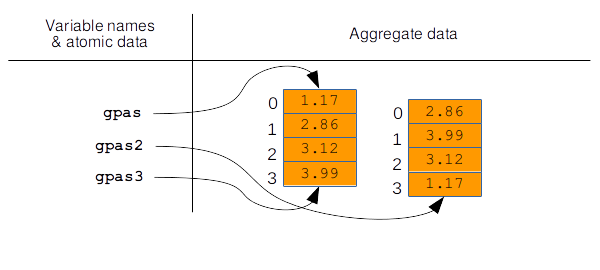
\includegraphics[width=0.9\textwidth]{dotSortArray.png}
\caption{The state of affairs after \texttt{.sort()}ing the \texttt{gpas} array in place.}
\label{fig:dotSortArray}
\end{figure}

\index{sorting@sorting (arrays)}
\index{sort@\texttt{np.sort()} (NumPy)}
\index{calling a function@``calling'' a function}
\index{passing an argument@``passing'' an argument}
The second option is to call the \texttt{np.sort()} function and pass an array
as an object. Like many Python functions, including the ones in the next
section, \texttt{np.sort()} \textit{returns a modified copy} of its argument
rather than changing it in place. To illustrate:

\index{Ravens, Baltimore}
\index{Patriots, New England}
\index{Broncos, Denver}
\index{Steelers, Pittsburgh}
\begin{Verbatim}[fontsize=\small,samepage=true,frame=single,framesep=3mm]
nfl_teams = np.array(["Ravens", "Patriots", "Broncos",
    "Chargers", "Steelers"])
sorted_teams = np.sort(nfl_teams)
print(nfl_teams)
print(sorted_teams)
\end{Verbatim}

\begin{Verbatim}[fontsize=\small,samepage=true,frame=leftline,framesep=5mm,framerule=1mm]
['Ravens' 'Patriots' 'Broncos' 'Chargers' 'Steelers']
['Broncos' 'Chargers' 'Patriots' 'Ravens' 'Steelers']
\end{Verbatim}

\index{return value}
Observe that the \texttt{nfl\_teams} variable, even though we passed it to
\texttt{np.sort()}, was not \textit{itself} sorted. The \texttt{sorted\_teams}
variable, on the other hand, \textit{is} alphabetically sorted, because we
assigned the return value from \texttt{np.sort()} to it. Again, the memory
picture is shown in Figure~\ref{fig:npSortArray}.

\index{on@``on''}
\begin{figure}[ht]
\centering
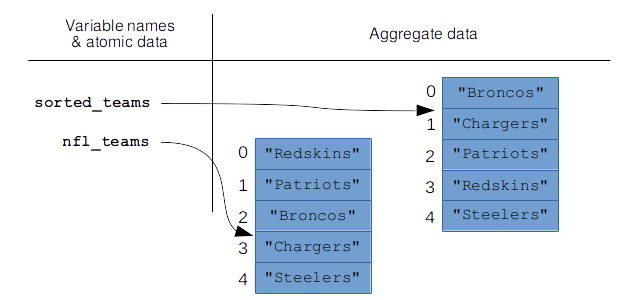
\includegraphics[width=0.9\textwidth]{npSortArray.png}
\medskip
\caption{Calling the \texttt{np.sort()} function (as opposed to calling the
\texttt{.sort()} method \textbf{on} the array) returns a sorted copy.}
\label{fig:npSortArray}
\end{figure}

To be clear, either one of these techniques can be used on \textit{any}
\texttt{ndarray}: whole numbers, real numbers, or text. I just chose to do real
numbers in the first example and text in the second. The difference between the
two is merely in what is affected: in one, the actual array in memory is
modified, and in the other, a modified copy is returned.

\section{More exotic array modifications}

\index{in place@``in place''}
Finally, there are lots of additional things you can do to an array to either
modify its structure or rearrange its contents. Here's a few.
\textbf{Important: all of the functions in this section return a modified copy
of the array you pass to it. They do \textit{not} change the array in place.}

\begin{itemize}
\itemsep.1em
\index{concatenating!arrays}
\index{append@\texttt{append()} (NumPy)}
\index{insert@\texttt{insert()} (NumPy)}
\index{delete@\texttt{delete()} (NumPy)}
\index{flip@\texttt{flip()} (NumPy)}
\index{reversing (an array)}
\item \texttt{np.append()} can be used to add a single element to the end of an
array, or to add an entire second array of elements to it. (In the latter case,
this is really \textbf{concatenation} of arrays.)
\item \texttt{np.insert()} is like the first form of \texttt{np.append()},
except it inserts in the middle (or the beginning).
\item \texttt{np.delete()} will remove an element of an array \textit{by
position}. In other words, you tell it which \textit{index number} to remove,
not which element.
\item \texttt{np.flip()} reverses the order of elements in an array.
\end{itemize}

These functions are all summarized in Figure~\ref{fig:handyNumPy}.

Remember that when you're calling a function like this -- which returns a
modified copy -- it is perfectly acceptable to store the return value
\textit{in the same variable} that you passed it. This is common if you don't
actually want to keep around the original:

\begin{Verbatim}[fontsize=\small,samepage=true,frame=single,framesep=3mm]
ice_cream_flavors = np.flip(ice_cream_flavors)
\end{Verbatim}

In this pattern, the net effect \textit{is} effectively to modify the array in
place, since you're making a reversed copy, and then assigning that reversed
copy to the same variable.

Anyway, here's some example code to illustrate the functions in this section:

\begin{Verbatim}[fontsize=\small,samepage=true,frame=single,framesep=3mm]
clowns = np.array(["Bozo", "Krusty"])
more_clowns = np.array(["Pennywise", "Skelton"])
more_clowns = np.insert(more_clowns, 1, "Happy Slappy")
all_clowns = np.append(clowns, more_clowns)
all_clowns = np.append(all_clowns, "Ronald McDonald")
all_clowns = np.flip(all_clowns)
all_clowns = np.delete(all_clowns, 2)
print("clowns is: {}".format(clowns))
print("more_clowns is: {}".format(more_clowns))
print("all_clowns is: {}".format(all_clowns))
\end{Verbatim}

\begin{Verbatim}[fontsize=\footnotesize,samepage=true,frame=leftline,framesep=5mm,framerule=1mm]
clowns is: ['Bozo' 'Krusty']
more_clowns is: ['Pennywise' 'Happy Slappy' 'Skelton']
all_clowns is: ['Ronald' 'Skelton' 'Pennywise' 'Krusty' 'Bozo']
\end{Verbatim}

% TODO: memory picture of the clowns


\section{Summary}

The table in Figure~\ref{fig:handyNumPy} gives the promised summary of
functions, methods, and operators in this chapter.

\setlength\extrarowheight{5pt}

\begin{figure}[ht]
\centering
\footnotesize
\begin{tabular}{c|p{3.1in}}
Function & Description \\
\hline

\texttt{len(}\textsl{arr}\texttt{)} & Get the number of elements in the array \textsl{arr}. \\

\textsl{arr}\texttt{[17]} & Get a specific element's value from the array \textsl{arr}. \\

\textsl{arr}\texttt{[8] =} (\textsl{something}) & Set a specific element of the array \textsl{arr}. \\

\textsl{arr} \texttt{+ 91} & Add a value to each element of \textsl{arr},
yielding a new array. (Also works with \texttt{-}, \texttt{*}, \texttt{/},
\textit{etc.}) \\

\textsl{arr1} \texttt{+} \textsl{arr2} & Add each pair of values in two arrays,
yielding a new array. (Also works with \texttt{-}, \texttt{*}, \texttt{/},
\textit{etc.}) \\

\textsl{arr1} = \textsl{arr2} & Make \textsl{arr1} point to the same data that
\textsl{arr2} points to. (\textit{Not} a copy!)\\

\textsl{arr1} = \textsl{arr2}\texttt{.copy()} & Make \textsl{arr1} point to a
new, independent copy of \textsl{arr2}. \\

\textsl{arr}\texttt{.sort()} & Sort the array \textsl{arr} \textbf{in place}. (Numerical or
alphabetical, depending on the \texttt{.dtype}.) \\

\texttt{np.sort(}\textsl{arr}) & Return a new array with the sorted elements
of \textsl{arr}. (Numerical or alphabetical, depending on the \texttt{.dtype}.)
\\

\texttt{np.append(}\textsl{arr}, \textsl{elem}\texttt{)} &
    Return a new array with \textsl{elem} tacked on to the end. \\

\texttt{np.append(}\textsl{arr1}, \textsl{arr2}\texttt{)} &
    Return a new array with the two arrays \textsl{arr1} and \textsl{arr2} concatenated. \\

\texttt{np.insert(}\textsl{arr}, \textsl{ind}, \textsl{val}\texttt{)} &
    Return a new array with the new value \textsl{val} inserted into position \textsl{ind} of \textsl{arr}. \\

\texttt{np.delete(}\textsl{arr}, \textsl{ind}\texttt{)} &
    Return a new array with the element at index \textsl{ind} removed from \textsl{arr}. \\

\texttt{np.flip(}\textsl{arr}\texttt{)} &
    Return a new array with \textsl{arr} in reverse order. \\
\end{tabular}
\bigskip
\caption{Handy NumPy functions, methods, and operators.}
\label{fig:handyNumPy}
\end{figure}

\pagebreak
\bigskip
\subsubsection{The answer}

\index{42 (Life, Universe, Everything)}
Oh, and the answer to the puzzle on p.~\pageref{indexTest} -- and also the
answer to Life, the Universe, and Everything, as it turns out -- is 42.

